\documentclass[tikz]{standalone}

\usepackage{tikz}
\usetikzlibrary{positioning} 


\begin{document}
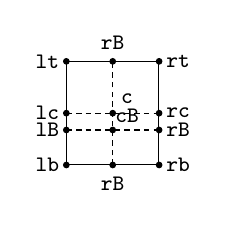
\begin{tikzpicture}

\fontsize{40}{40}\selectfont
\node [draw=black, text=white] (ch) {Q};

\fontsize{8}{8}\selectfont
\ttfamily
% \foreach \label \pos / \xshift / \yshift in {rB / ch.base east / 2ex / 0ex,
% rc / ch.east / 2ex / 0ex,
% rt / ch.north east / 2ex / 0ex,
% rb / ch.south east / 2ex / 0ex,
% lB / ch.base west / 2ex / 0ex,
% lc / ch.west / 2ex / 0ex,
% lt / ch.north west / 2ex / 0ex,
% lb / ch.south west / 2ex / 0ex,
% cb / ch.north / 2ex / 0ex,
% ct / ch.south / 2ex / 0ex,
% ct / ch.base / 2ex / 0ex,
% ct / ch / 2ex / 0ex,
% }
% \filldraw (\pos east) circle (1pt); \node at ([xshift=\xshift ,yshift=\yshift]\pos) {\label};

\filldraw (ch.base east) circle (1pt); \node at ([xshift=2ex]ch.base east) {rB};
\filldraw (ch.east) circle (1pt); \node at ([xshift=2ex]ch.east) {rc};
\filldraw (ch.north east) circle (1pt); \node at ([xshift=2ex]ch.north east) {rt};
\filldraw (ch.south east) circle (1pt); \node at ([xshift=2ex]ch.south east) {rb};
\filldraw (ch.base west) circle (1pt); \node at ([xshift=-2ex]ch.base west) {lB};
\filldraw (ch.west) circle (1pt); \node at ([xshift=-2ex]ch.west) {lc};
\filldraw (ch.north west) circle (1pt); \node at ([xshift=-2ex]ch.north west) {lt};
\filldraw (ch.south west) circle (1pt); \node at ([xshift=-2ex]ch.south west) {lb};
\filldraw (ch.north) circle (1pt); \node at ([yshift=2ex]ch.north) {rB};
\filldraw (ch.south) circle (1pt); \node at ([yshift=-2ex]ch.south) {rB};
\filldraw (ch.base) circle (1pt); \node at ([xshift=1.5ex, yshift=1.5ex]ch.base) {cB};
\filldraw (ch) circle (1pt); \node at ([xshift=1.5ex, yshift=1.5ex]ch) {c};

\draw [dash pattern=on 2pt off 1.5pt] (ch.south) -- (ch.north);
\draw [dash pattern=on 2pt off 1.5pt] (ch.west) -- (ch.east);
\draw [dash pattern=on 2pt off 1.5pt] (ch.base west) -- (ch.base east);



\end{tikzpicture}
\end{document}

% references
% - https://tex.stackexchange.com/questions/147052/tikz-how-to-set-a-node-on-an-exact-position-on-a-line
% - https://stackoverflow.com/questions/2939450/get-height-on-a-block-of-latex-output
% - https://tex.stackexchange.com/questions/78288/how-to-fix-tikz-nodes-height-with-heightof
% - https://tex.stackexchange.com/questions/171426/increments-in-foreach-loop-with-two-variables-tikz